\chapter{综合应用}
当你来到这一章节时,你应该对Linux内核的主要组成部分有了清晰的了解,对每个部分的修改效果应该也熟悉了。
在这个基础上,我们进一步探讨我们的综合应用。

\section{使用RDMA的远程内存Swap}
在这个项目中,你需要实现一个简单的使用远程内存的交换分区(swap)。具体而言,当缺页异常发生时,你需要使用RDMA访问远程内存将页面换到本地。如果远程页面不存在,你需要寻找本地交换文件中寻找这个目标页面。在两者都不存在的情况下,应当给出一个内存错误(如同访问非法地址的错误)。
\subsection{指标}
\paragraph*{项目形态。}
你的项目最终的形态应当符合以下指标:
\begin{enumerate}
    \item 将交换分区的内存页面通过RDMA存储到远程内存上。
    \item 设定一个可调整的比例决定远程内存和本地内存的比例。
    \item 对应用无感。
\end{enumerate}

\paragraph*{基础评测指标。}
项目的基础评测指标如下:
\begin{enumerate}
    \item 使用\texttt{memcached}~\cite{fitzpatrick2004distributed}存储一系列数据(YCSB~\cite{cooper2010benchmarking})在使用50\%远程内存时在50\%能够产生一个显著的时间差。
    \item 使用RDMA的交换时间需要比磁盘交换更短。
\end{enumerate}

对于基础评测指标,一个简单的示意图如图~\ref{fig:mixed:rdma-examples}所示。

\begin{figure}[h]
\centering
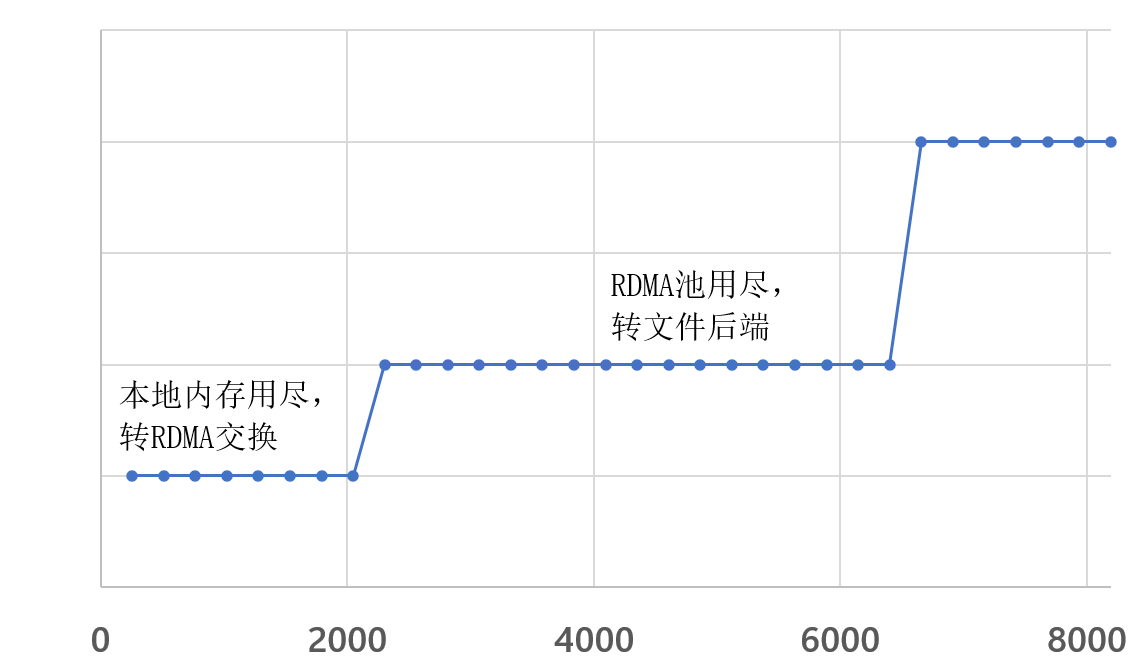
\includegraphics[scale=0.5]{figure/mixed-figures/RDMA-example.png}
\caption{RDMA和文件混合交换分区下的内存访问量同时间的示意图。图中假设本地内存为2048MB,RDMA内存约4096MB。相对时间仅为示意图,不代表真实场景数据。}
\label{fig:mixed:rdma-examples}
\end{figure}

\paragraph*{进阶指标。}
在基础评测的指标上,结合内存访问的特点,实现页预取和交换,目标发生尽可能少的缺页异常。

\subsection{快速上手和实现重点提示}
本项目的核心包括两个部分,内存管理和RDMA的访问。对于内存管理部分,需要修改原有系统的Page Fault处理流程。RDMA部分则需要维护RDMA连接确保发生缺页异常时向远端设备发起RDMA读写请求。

\paragraph*{内存管理。} 缺页异常发生后,操作系统需要确认这个页位于什么地方(是在内存中但是页表没有映射?还是这个页已经被交换到磁盘设备?或是这个页根本不存在?)。传统的顺序流程可以在体系结构下的\texttt{mm/fault.c}中找到相关的代码。加入RDMA后,需要保证RDMA部分不能被换出,并且加入对RDMA内存的搜索。

\paragraph*{RDMA管理。} RDMA的通信与不同的以太网通信不同。为了保证传输的速度,RDMA没有使用套接字(Socket)抽象。取而代之的是两大类Verbs(Memory Verbs和Message Verbs)这两大类的Verbs具体包含:Read(远程主机读取部分内存)、Write(数据写到远端主机)、Atomic(原子操作);Send(把数据发送到远程 QP 的接收队列里)、Receive(接收主机被告知接收到数据缓冲)。具体的管理可以参考以下链接:(中文)\url{https://zhuanlan.zhihu.com/p/649468433}(英语官方原版)\url{https://academy.nvidia.com/en/course/rdma-programming-intro/?cm=446}

\paragraph*{特殊点提示。}
\begin{itemize}
    \item 多线程的访问安全性:多个进程同时发生缺页异常在远端的处理过程;
    \item RDMA内存的管理:减少远端内存中的内存碎片。
\end{itemize}

\section{用户程序嵌入内核执行}
用户程序执行时需要通过系统调用(syscall)调用特权系统服务,每一次系统调用都有上下文切换的开销,从而使得密集调用系统调用的程序产生额外的开销。
一种简单的优化方法是将含有系统调用的程序嵌入内核执行,从而避免上下文切换。
这一更改实际上给内核打了很多的“洞”,忽略了内核的权限隔离,因此是不安全的。
我们深入之后会发现,这一想法的核心其实是一部分上下文权限隔离对程序而言过强了,程序没有用到对应的功能因此也不需要对应的隔离。
在这个基础上,我们可以通过为一些简单程序设计内核中隔离他们程序的方案。
具体而言,通过修改fork的过程将程序直接嵌入内核空间,增加一些特殊的机制(你自定义的机制,可以是页表、MPK等)实现该段代码在内核中仅能访问特定内存(相当于自己的地址空间)。
假设程序不是恶意的,因此不需要你考虑控制流完整性,但是需要注意代码的映射区域。
同时假设在这项作业中程序已经被编译为位置无关代码。


\subsection{指标}
\paragraph*{项目形态。}
你的项目最终的形态应当符合以下指标:
\begin{enumerate}
    \item 将一段程序嵌入到内核态执行,程序本身无需修改。
    \item 程序仅能访问自己的内存区间,而不能访问内核的其他数据结构。
\end{enumerate}

\paragraph*{基础评测指标。}
项目的基础评测指标如下:
\begin{enumerate}
    \item 一段仅包含一系列系统调用的程序可以进入内核实现吞吐的显著提升。
    \item 程序访问非法内存应当退出当前程序的执行,给出错误信息(可以在内核日志)并且不影响当前内核的执行。
    \item 支持多线程程序的执行,不影响多线程程序的可扩展性。
\end{enumerate}


\paragraph*{进阶指标。}
在基础评测的指标上,支持带有多个用户库文件的用户程序进入内核执行。

\subsection{快速上手和实现重点提示}
本项目的核心包括两个部分,代码启动阶段(fork)和执行阶段(exec)。

\paragraph*{启动阶段}
启动阶段用户程序并没有执行,核心需要考虑的部分是如何映射用户段的代码到内核空间,以及如何设置权限隔离的初始状态。
此外,需要在启动阶段拦截系统调用,确保系统调用转换为内核态的函数跳转。


\paragraph*{执行阶段}
执行阶段最核心的是在遇到错误的时候如何修正错误的状态,从而避免嵌入内核的程序崩溃内核。

\paragraph*{特殊点提示。}
\begin{itemize}
    \item 多线程执行:与内核线程的绑定执行关系;
    \item 内核状态的保护:防止单个程序崩溃整个内核。
\end{itemize}

\section{内核空间下的内存磁盘}
随着硬件的发展,内存的价格已经显著下降。
内存的访问速度非常快,可以作为一部分反复读写的文件的临时存储。
这一部分是用户空间下的内存磁盘的进一步延伸。


\subsection{指标}
\paragraph*{项目形态。}
你的项目最终的形态应当符合以下指标:
\begin{enumerate}
    \item 将一段内存空间作为磁盘空间映射给内核。
    \item 映射的磁盘空间可以进行文件读写和文件夹创建。
    \item 注册为一个磁盘设备而非文件系统。
\end{enumerate}

\paragraph*{基础评测指标。}
项目的基础评测指标如下:
\begin{enumerate}
    \item 使用\texttt{dd}一次性创建一个大文件的开销足够小(需要接近内存的读写速度)。
    \item 多次创建删除文件之后实际存储容量始终保持一致。
\end{enumerate}


\paragraph*{进阶指标。}
在基础评测的指标上,减小文件元数据的开销大小。

\subsection{快速上手和实现重点提示}
本项目的核心是内存空间的映射和分区管理。
与映射在用户空间不同,内核空间的映射需要保证用于虚拟磁盘的数据不能破坏内核数据的正确性。
此外,用户空间可以通过\texttt{fuse}实现用户态的分区访问。在内核中,该模块需要实现为内核模块,因此需要符合内核的一系列数据接口。

\paragraph*{特殊点提示。}
\begin{itemize}
    \item 多线程执行:多线程读写保证数据的一致性。
    \item 文件碎片:文件的碎片应该尽可能少。
\end{itemize}

\section{机密虚拟机Trapless的宿主协同内存管理}
机密虚拟机的一个核心是内存需要加密以防止宿主可以获取到虚拟机内存造成数据泄露,然而这样的安全措施也造成了宿主机无法感知虚拟机内的内存情况,内存分配无法最优化。
一种方式是虚拟机内核主动向宿主机的虚拟机管理器发起调用引导宿主机按照一定的偏好管理内存。
这种方式需要下陷到宿主机的虚拟机管理器,有较大的切换开销。
请设计一种机制,以不下陷的方式引导宿主机的按照一定偏好管理内存。



\subsection{指标}
\paragraph*{项目形态。}
你的项目最终的形态应当符合以下指标:
\begin{enumerate}
    \item 不修改虚拟机内应用程序,允许修改虚拟机管理器和虚拟机内的内核。
    \item 指示内存偏好时不发生下陷。
\end{enumerate}

\paragraph*{基础评测指标。}
项目的基础评测指标如下:
\begin{enumerate}
    \item 使用内存密集型任务在机密虚拟机内部设置特定内存位置后计算速度和用户态的读写速度一致。
\end{enumerate}


\subsection{快速上手和实现重点提示}
本项目的指标较少,因为核心代码需要较大的修改,包括三个部分:宿主机的内核、虚拟机的内核、宿主机的虚拟机管理器。
宿主机内核需要设定特殊的接口管理加密的内存页面。
虚拟机内核需要修改实现无下陷与宿主机的虚拟机管理器进行交互。
宿主机的虚拟机内存管理器需要增加接收虚拟机内核的特殊内存偏好参数并且传递给宿主机。

\paragraph*{特殊点提示。}
\begin{itemize}
    \item 虚拟机下陷的处理。
    \item 共享内存页的管理。
    \item 宿主机的内存管理。
\end{itemize}